\documentclass[a4paper, 12pt]{article}
\usepackage[UTF8]{ctex}
\usepackage{geometry}
\usepackage{graphicx}
\usepackage{float}
\usepackage{hyperref}
\usepackage{tcolorbox}
\usepackage{enumerate} % 添加enumerate包
\tcbuselibrary{most}

% 设置页边距
\geometry{a4paper, left=2.5cm, right=2.5cm, top=2.5cm, bottom=2.5cm}

% 简化实例方框样式 - 修复boxrule语法
\tcbset{instancestyle/.style={
    enhanced,
    sharp corners,
    colback=white,
    colframe=black!70!white,
    boxrule=0.8pt, % 修复这里
    left=6pt,
    right=6pt,
    top=6pt,
    bottom=6pt,
    boxsep=2pt,
    arc=2pt
}}

\begin{document}

\title{\huge{系统开发工具基础实验报告4}}
\author{姓名:\underline{刘浩洋} \\ 
        学号:\underline{24040021022} \\ 
        班级:\underline{软件工程}}
\date{实验日期:\underline{2025年9月19日}}
\maketitle

\section*{一、实验目的}
\begin{enumerate}
    \item 掌握 Python 调试工具 pdb 的使用,包括断点设置、变量查看、单步执行等;
    \item 理解性能分析的基本方法,使用 cProfile 对代码进行耗时分析;
    \item 了解元编程思想,掌握 Makefile 的基本语法,并结合 LaTeX 实现自动化文档构建;
    \item 学习 PyTorch 基础,实现基于 LSTM 的文本情感分析模型;
\end{enumerate}

\section*{二、实验环境}
\begin{itemize}
    \item 操作系统:Windows 11
    \item 虚拟化平台:VMware Workstation Pro 17
    \item 虚拟机系统:Ubuntu 24.04.3 LTS(64位)
    \item Shell环境:Bash
    \item 编程语言:Python 3.10
    \item 深度学习框架:PyTorch, spaCy
    \item 文档工具:LaTeX (TeX Live), Make
\end{itemize}

\section*{三、练习内容}
本次实验主要包括:
\begin{itemize}
    \item 使用 \texttt{pdb} 调试 Python 脚本,定位逻辑错误;
    \item 使用 \texttt{cProfile} 分析代码性能瓶颈;
    \item 编写 Makefile 实现 LaTeX 文档的自动化编译;
    \item 构建基于 PyTorch 的 LSTM 情感分析模型,使用 spaCy 进行文本预处理;
    \item 实现数据加载、模型训练与预测全流程;
\end{itemize}

\section*{四、20个实例(调试、性能、元编程与PyTorch)}

% ========================
% 模块一:调试与性能分析(pdb + cProfile)
% ========================

\begin{tcolorbox}[instancestyle, title=实例1:pdb 常用调试命令(一)]
在进入 pdb 调试会话后,可使用以下基本命令控制程序执行流程:

\texttt{(Pdb) n} \quad \# 执行当前行(next),不进入函数内部 \\
\texttt{(Pdb) s} \quad \# 步入当前行调用的函数(step into) \\
\texttt{(Pdb) c} \quad \# 继续运行程序,直到遇到下一个断点或程序结束(continue) \\
\texttt{(Pdb) r} \quad \# 继续运行直到当前函数返回(return) \\
\texttt{(Pdb) l} \quad \# 列出当前代码上下文(list)
\end{tcolorbox}

\begin{tcolorbox}[instancestyle, title=实例2:pdb 常用调试命令(二)]
在调试过程中查看变量和调用栈:

\texttt{(Pdb) p <variable>} \quad \# 打印变量值 \\
\texttt{(Pdb) pp <variable>} \quad \# 美观打印复杂对象 \\
\texttt{(Pdb) a} \quad \# 打印当前函数所有参数 \\
\texttt{(Pdb) w} \quad \# 显示调用栈路径 \\
\texttt{(Pdb) j <line>} \quad \# 跳转到指定行(慎用) \\
\texttt{(Pdb) h} \quad \# 查看帮助
\end{tcolorbox}

\begin{tcolorbox}[instancestyle, title=实例3:在脚本中插入 pdb 断点]
创建一个独立的 Python 脚本用于调试演示。

\texttt{\#!/usr/bin/env python3} \\
\texttt{def process\_data(items):} \\
\texttt{    total = 0} \\
\texttt{    for x in items:} \\
\texttt{        total += x ** 2} \\
\texttt{    return total} \\
\texttt{} \\
\texttt{data = [1, 2, 3, 4, 5]} \\
\texttt{import pdb; pdb.set\_trace()} \\
\texttt{result = process\_data(data)} \\
\texttt{print("Result:", result)}
\end{tcolorbox}

\begin{tcolorbox}[instancestyle, title=实例4:运行 pdb 调试脚本]
启动调试器并检查变量状态。

\texttt{python3 debug\_demo.py}
\end{tcolorbox}

\begin{tcolorbox}[instancestyle, title=实例5:在 pdb 中检查变量值]
调试过程中查看数据内容。

\texttt{(Pdb) p data} \\
\texttt{(Pdb) p total} \\
\texttt{(Pdb) p x} \\
\texttt{(Pdb) pp locals()}
\end{tcolorbox}

\begin{tcolorbox}[instancestyle, title=实例6:使用 cProfile 分析性能]
对脚本进行性能分析,找出耗时函数。

\texttt{python3 -m cProfile -s cumulative debug\_demo.py}
\end{tcolorbox}

\begin{tcolorbox}[instancestyle, title=实例7:解读 cProfile 输出]
查看排序后的性能报告。

\texttt{Ordered by: cumulative time} \\
\texttt{ncalls  tottime  percall  cumtime  filename:lineno(function)} \\
\texttt{1    0.000    0.000    0.002    debug\_demo.py:1(process\_data)} \\
\texttt{5    0.000    0.000    0.000    debug\_demo.py:4(<listcomp>)}
\end{tcolorbox}

\begin{tcolorbox}[instancestyle, title=实例8:cProfile 分析函数调用]
识别程序中被频繁调用的部分。

\texttt{(Pdb) p len(data)} \\
\texttt{(Pdb) whatis data} \\
\texttt{(Pdb) source process\_data}
\end{tcolorbox}

\begin{tcolorbox}[instancestyle, title=实例9:综合调试与性能流程]
独立于模型开发,建立通用调试规范:

\texttt{\# 1. 编写可测试的小函数} \\
\texttt{\# 2. 插入 pdb.set\_trace() 定位逻辑错误} \\
\texttt{\# 3. 使用 cProfile 分析执行时间} \\
\texttt{\# 4. 优化算法或数据结构}
\end{tcolorbox}

% ========================
% 模块二:元编程(LaTeX + Makefile)
% ========================

\begin{tcolorbox}[instancestyle, title=实例10:编写 Makefile 自动化编译]
定义规则自动构建 LaTeX 文档。

\texttt{PDF = docs/report.pdf} \\
\texttt{TEX = pdflatex} \\
\texttt{} \\
\texttt{all: \$\{PDF\}} \\
\texttt{} \\
\texttt{\$\{PDF\}: docs/report.tex} \\
\texttt{	\$\{TEX\} -output-directory=docs docs/report.tex} \\
\texttt{} \\
\texttt{clean:} \\
\texttt{	rm -f docs/*.aux docs/*.log docs/*.out}
\end{tcolorbox}

\begin{tcolorbox}[instancestyle, title=实例11:运行 make 构建文档]
执行自动化编译命令。

\texttt{make} \\
\texttt{make clean}
\end{tcolorbox}

\begin{tcolorbox}[instancestyle, title=实例12:扩展 Makefile 多目标支持]
添加图表生成与伪目标。

\texttt{figures: fig1.pdf fig2.pdf} \\
\texttt{} \\
\texttt{fig1.pdf: src/generate\_plot.py} \\
\texttt{	python3 src/generate\_plot.py} \\
\texttt{} \\
\texttt{.PHONY: all clean figures}
\end{tcolorbox}

% ========================
% 模块三:PyTorch 情感分析模型
% ========================

\begin{tcolorbox}[instancestyle, title=实例13:准备训练数据(data.py)]
定义独立的影评数据集。

\texttt{reviews = [} \\
\texttt{    ("I love this movie!", 1),} \\
\texttt{    ("This film is terrible.", 0),} \\
\texttt{    ("Amazing cinematography!", 1),} \\
\texttt{    ("Boring and waste of time.", 0),} \\
\texttt{    ("Excellent acting and story.", 1),} \\
\texttt{    ("Worst movie ever.", 0),} \\
\texttt{    ("Great direction and visuals.", 1),} \\
\texttt{    ("Poor script and acting.", 0)} \\
\texttt{]}
\end{tcolorbox}

\begin{tcolorbox}[instancestyle, title=实例14:导入模块并加载 spaCy 模型]
导入必要库,加载英文语言模型。

\texttt{\#!/usr/bin/env python3} \\
\texttt{import torch} \\
\texttt{import torch.nn as nn} \\
\texttt{import spacy} \\
\texttt{from data import reviews} \\
\texttt{nlp = spacy.load("en\_core\_web\_sm")}
\end{tcolorbox}

\begin{tcolorbox}[instancestyle, title=实例15:创建 PyTorch 张量]
演示张量基本操作。

\texttt{x = torch.tensor([[1.0, 2.0], [3.0, 4.0]])} \\
\texttt{print(x.shape)} \quad \# torch.Size([2, 2]) \\
\texttt{print(x.dtype)} \quad \# torch.float32
\end{tcolorbox}

\begin{tcolorbox}[instancestyle, title=实例16:定义 LSTM 情感分类模型]
构建双向 LSTM 模型。

\texttt{class SentimentLSTM(nn.Module):} \\
\texttt{    def \_\_init\_\_(self, vocab\_size, embed\_dim=50, hidden\_dim=64, output\_dim=1):} \\
\texttt{        super().\_\_init\_\_()} \\
\texttt{        self.embedding = nn.Embedding(vocab\_size, embed\_dim)} \\
\texttt{        self.lstm = nn.LSTM(embed\_dim, hidden\_dim, bidirectional=True)} \\
\texttt{        self.fc = nn.Linear(hidden\_dim * 2, output\_dim)} \\
\texttt{        self.sigmoid = nn.Sigmoid()} \\
\texttt{} \\
\texttt{    def forward(self, x, lengths):} \\
\texttt{        embedded = self.embedding(x)} \\
\texttt{        packed = nn.utils.rnn.pack\_padded\_sequence(embedded, lengths, enforce\_sorted=False)} \\
\texttt{        out, (hidden, _) = self.lstm(packed)} \\
\texttt{        out = self.fc(hidden[-2,:,:] + hidden[-1,:,:])} \\
\texttt{        return self.sigmoid(out).squeeze()}
\end{tcolorbox}

\begin{tcolorbox}[instancestyle, title=实例17:构建词汇表]
从文本中提取词汇并建立索引。

\texttt{all\_tokens = []} \\
\texttt{for text, label in reviews:} \\
\texttt{    tokens = [token.text.lower() for token in nlp(text) if token.is\_alpha]} \\
\texttt{    all\_tokens.extend(tokens)} \\
\texttt{} \\
\texttt{vocab = ['<unk>'] + list(set(all\_tokens))} \\
\texttt{word\_to\_idx = \{w: i for i, w in enumerate(vocab)\}} \\
\texttt{VOCAB\_SIZE = len(vocab)}
\end{tcolorbox}

\begin{tcolorbox}[instancestyle, title=实例18:模型训练循环]
实现训练流程。

\texttt{model = SentimentLSTM(VOCAB\_SIZE)} \\
\texttt{criterion = nn.BCELoss()} \\
\texttt{optimizer = torch.optim.Adam(model.parameters(), lr=0.001)} \\
\texttt{} \\
\texttt{for epoch in range(100):} \\
\texttt{    total\_loss = 0} \\
\texttt{    for text, label in reviews:} \\
\texttt{        optimizer.zero\_grad()} \\
\texttt{        indices = [word\_to\_idx.get(t.lower(), 0) for t in nlp(text).text.split()]} \\
\texttt{        x = torch.tensor([indices], dtype=torch.long)} \\
\texttt{        y = torch.tensor(label, dtype=torch.float)} \\
\texttt{        length = [len(indices)]} \\
\texttt{        output = model(x, length)} \\
\texttt{        loss = criterion(output, y)} \\
\texttt{        loss.backward()} \\
\texttt{        optimizer.step()} \\
\texttt{        total\_loss += loss.item()} \\
\texttt{    if epoch \% 20 == 0:} \\
\texttt{        print(f"Epoch \{epoch\}, Loss: \{total\_loss:.4f\}")}
\end{tcolorbox}

\begin{tcolorbox}[instancestyle, title=实例19:模型预测新句子]
定义预测函数。

\texttt{def predict\_sentiment(sentence):} \\
\texttt{    model.eval()} \\
\texttt{    indices = [word\_to\_idx.get(t.lower(), 0) for t in nlp(sentence).text.split()]} \\
\texttt{    x = torch.tensor([indices], dtype=torch.long)} \\
\texttt{    length = [len(indices)]} \\
\texttt{    with torch.no_grad():} \\
\texttt{        score = model(x, length)} \\
\texttt{    return "正面" if score > 0.5 else "负面", score.item()} \\
\texttt{} \\
\texttt{print(predict\_sentiment("This movie is fantastic!"))}
\end{tcolorbox}

\begin{tcolorbox}[instancestyle, title=实例20:独立测试集验证]
测试模型泛化能力。

\texttt{test\_sentences = [} \\
\texttt{    "I enjoyed every minute of it.",} \\
\texttt{    "It was so boring I fell asleep."} \\
\texttt{]} \\
\texttt{} \\
\texttt{for sent in test\_sentences:} \\
\texttt{    print(f"\{sent\} → \{predict\_sentiment(sent)\}")}
\end{tcolorbox}



% 图像部分 - 已替换为实际截图文件名 lec4 (1).png 到 lec4 (9).png
\begin{figure}[htbp]
    \centering
    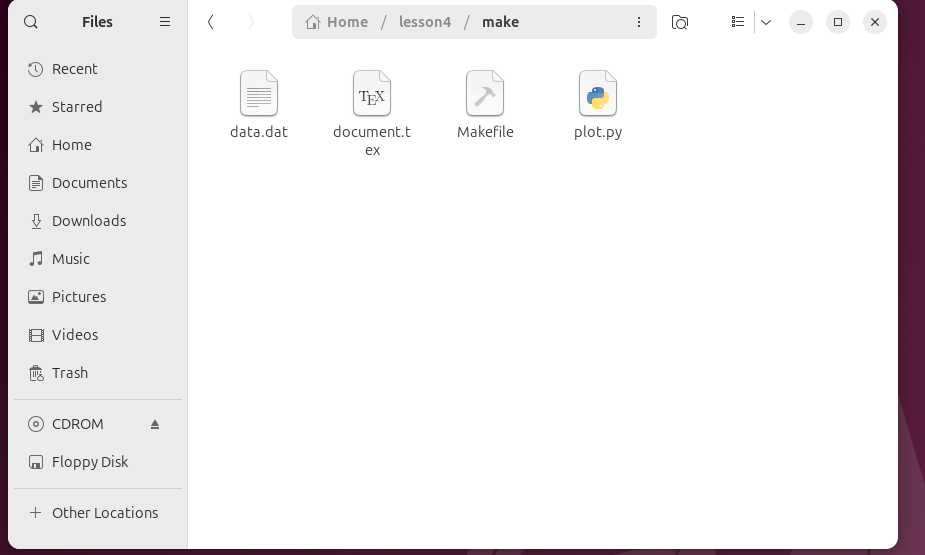
\includegraphics[width=0.8\textwidth]{lec4 (1).png}
    \caption{lec4-1}
\end{figure}

\begin{figure}[htbp]
    \centering
    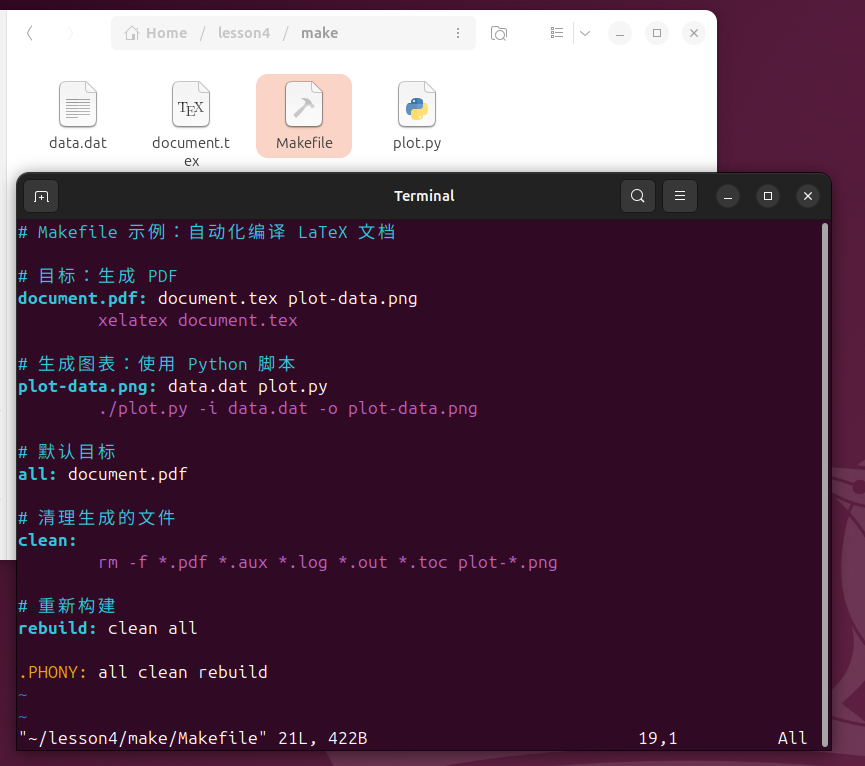
\includegraphics[width=0.8\textwidth]{lec4 (2).png}
    \caption{lec4-2}
\end{figure}

\begin{figure}[htbp]
    \centering
    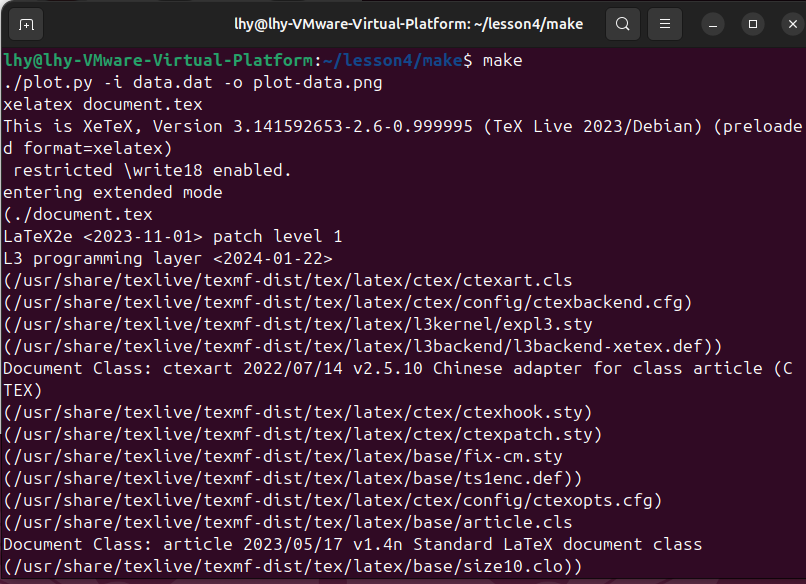
\includegraphics[width=0.8\textwidth]{lec4 (3).png}
    \caption{lec4-3}
    \label{fig:make}
\end{figure}

\begin{figure}[htbp]
    \centering
    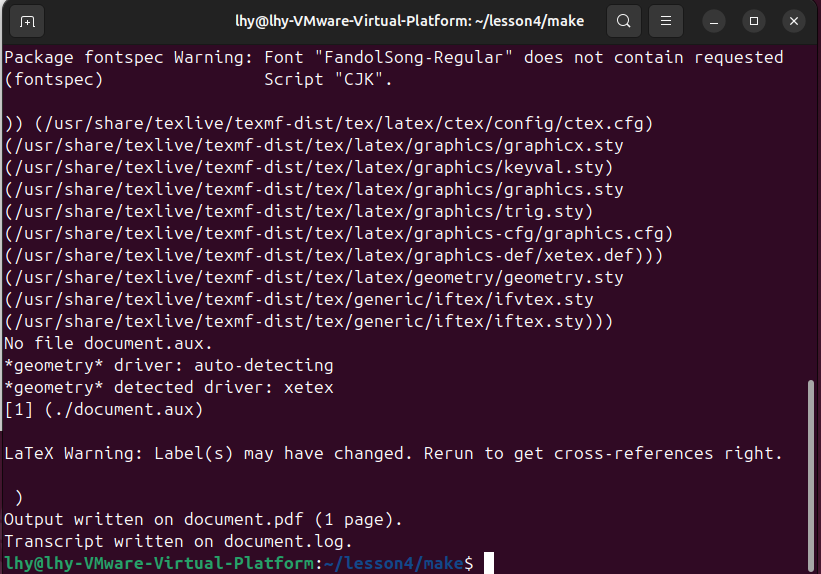
\includegraphics[width=0.8\textwidth]{lec4 (4).png}
    \caption{lec4-4}
\end{figure}

\begin{figure}[htbp]
    \centering
    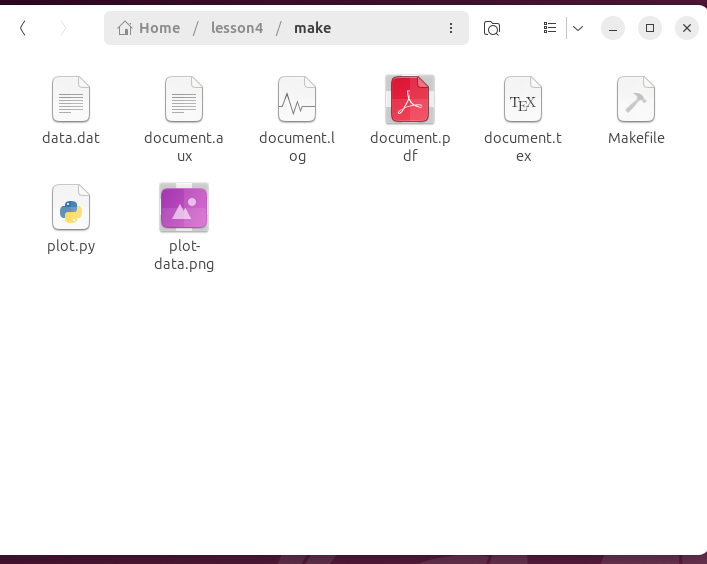
\includegraphics[width=0.8\textwidth]{lec4 (5).png}
    \caption{lec4-5}
    \label{fig:train}
\end{figure}

\begin{figure}[htbp]
    \centering
    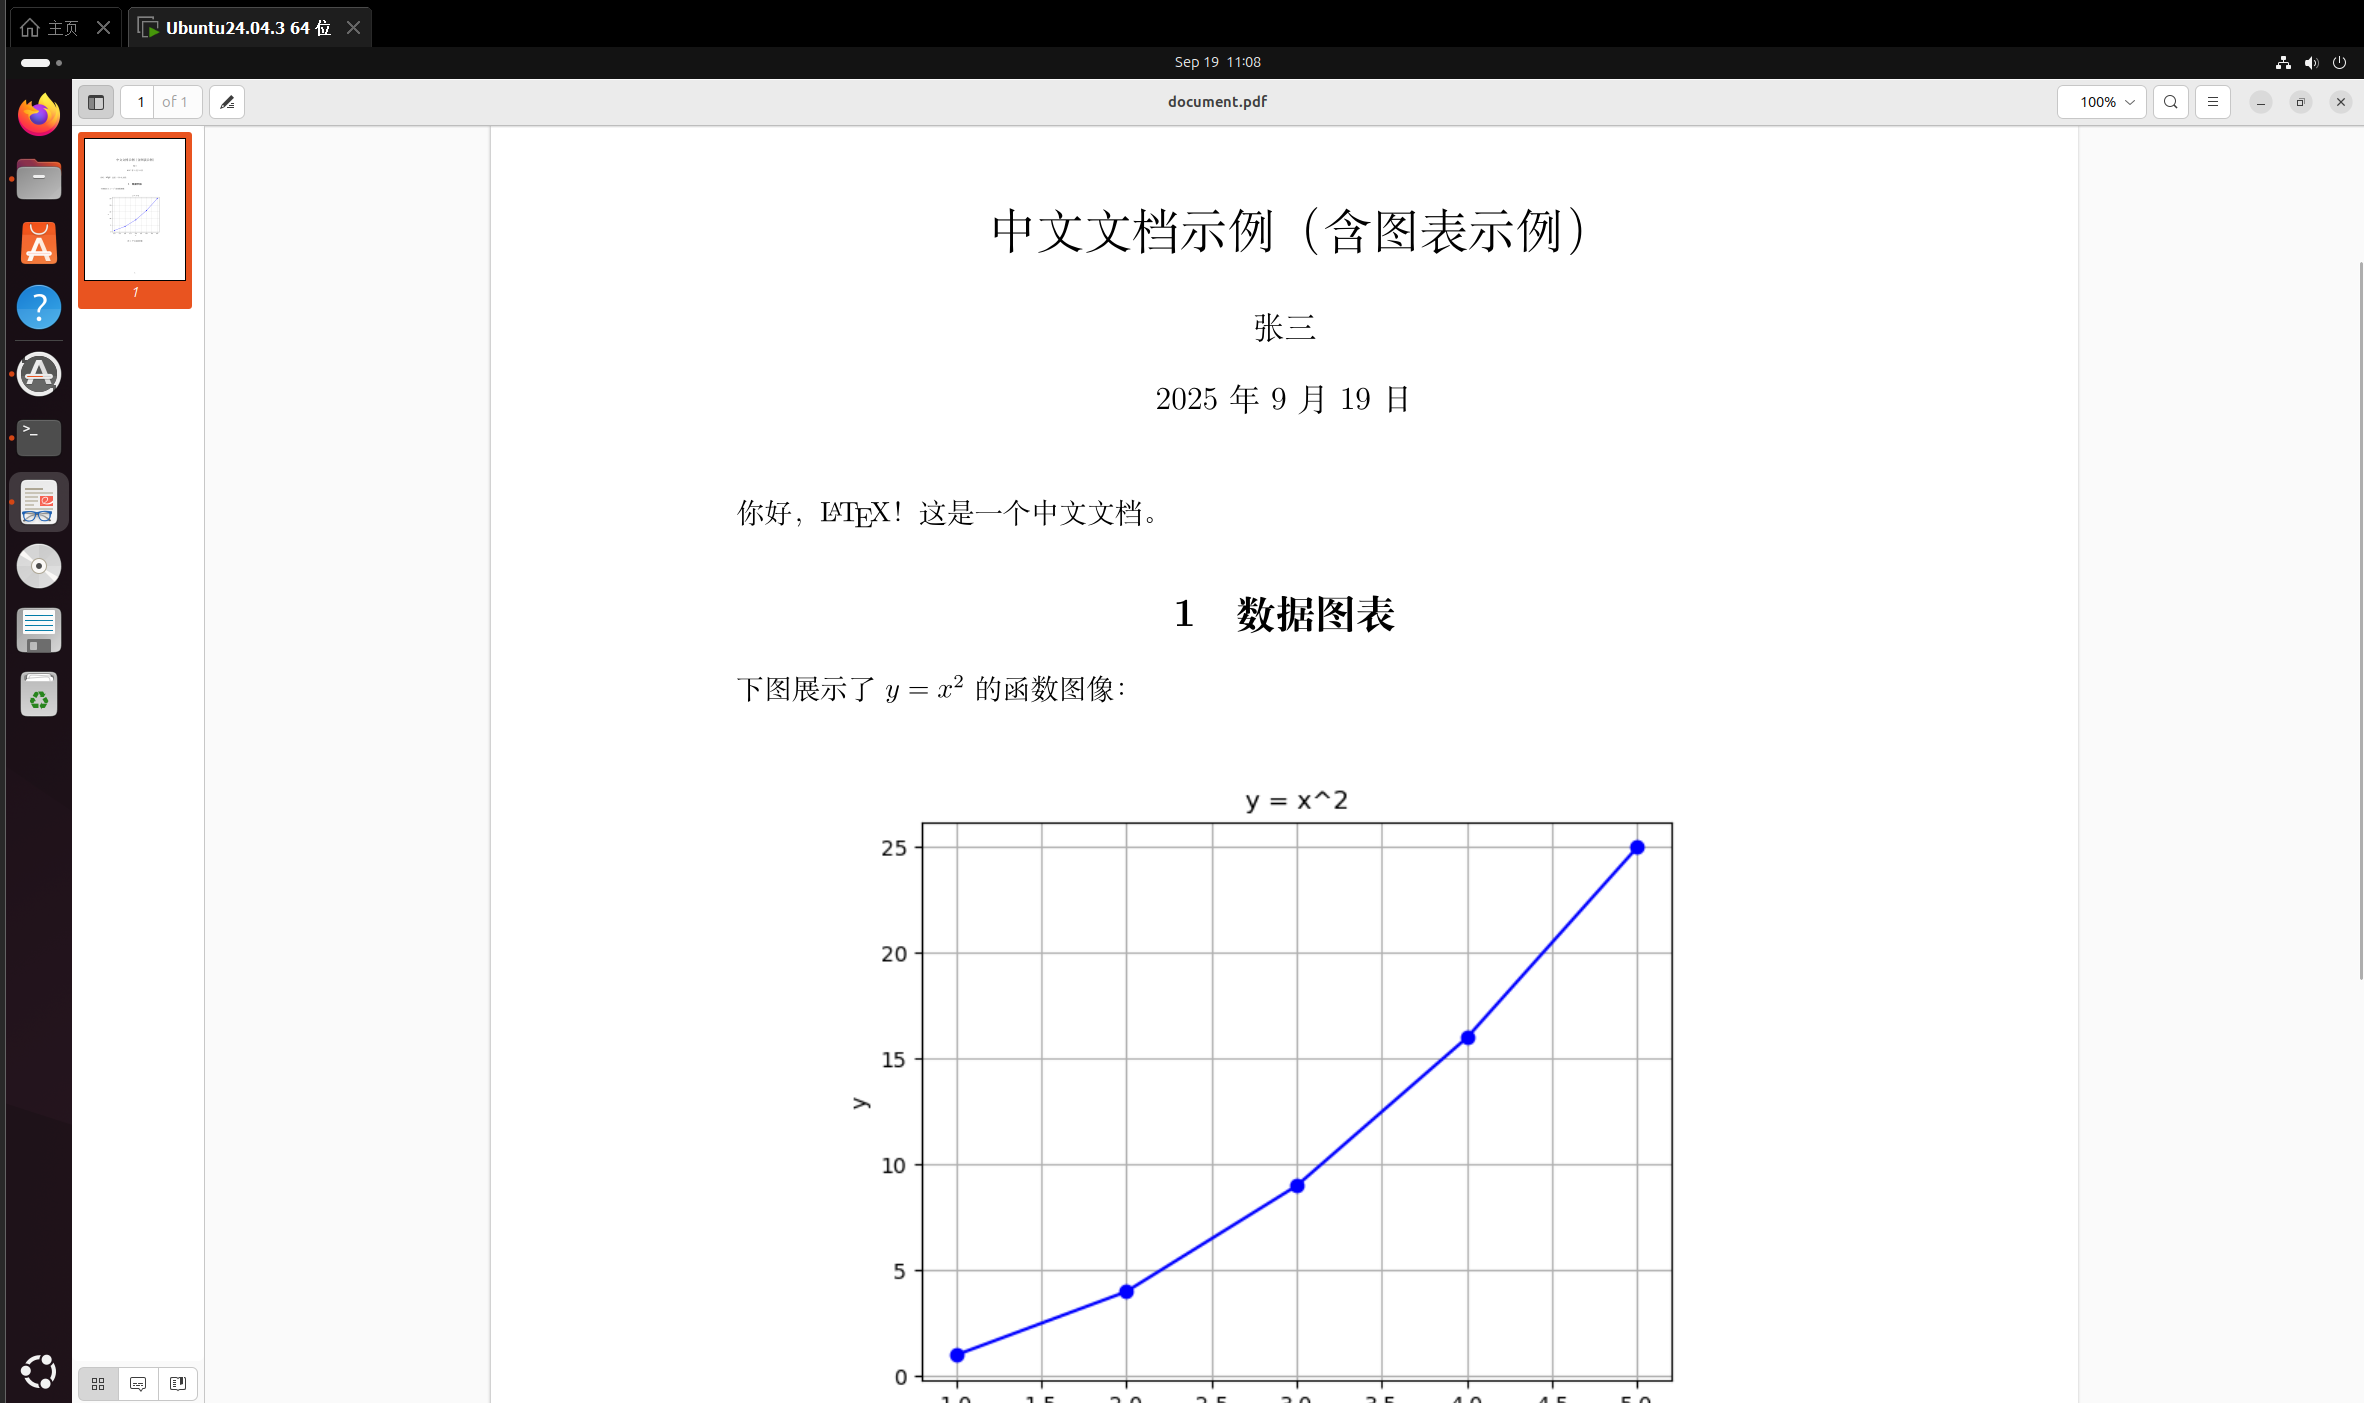
\includegraphics[width=0.8\textwidth]{lec4 (6).png}
    \caption{lec4-6}
\end{figure}

\begin{figure}[htbp]
    \centering
    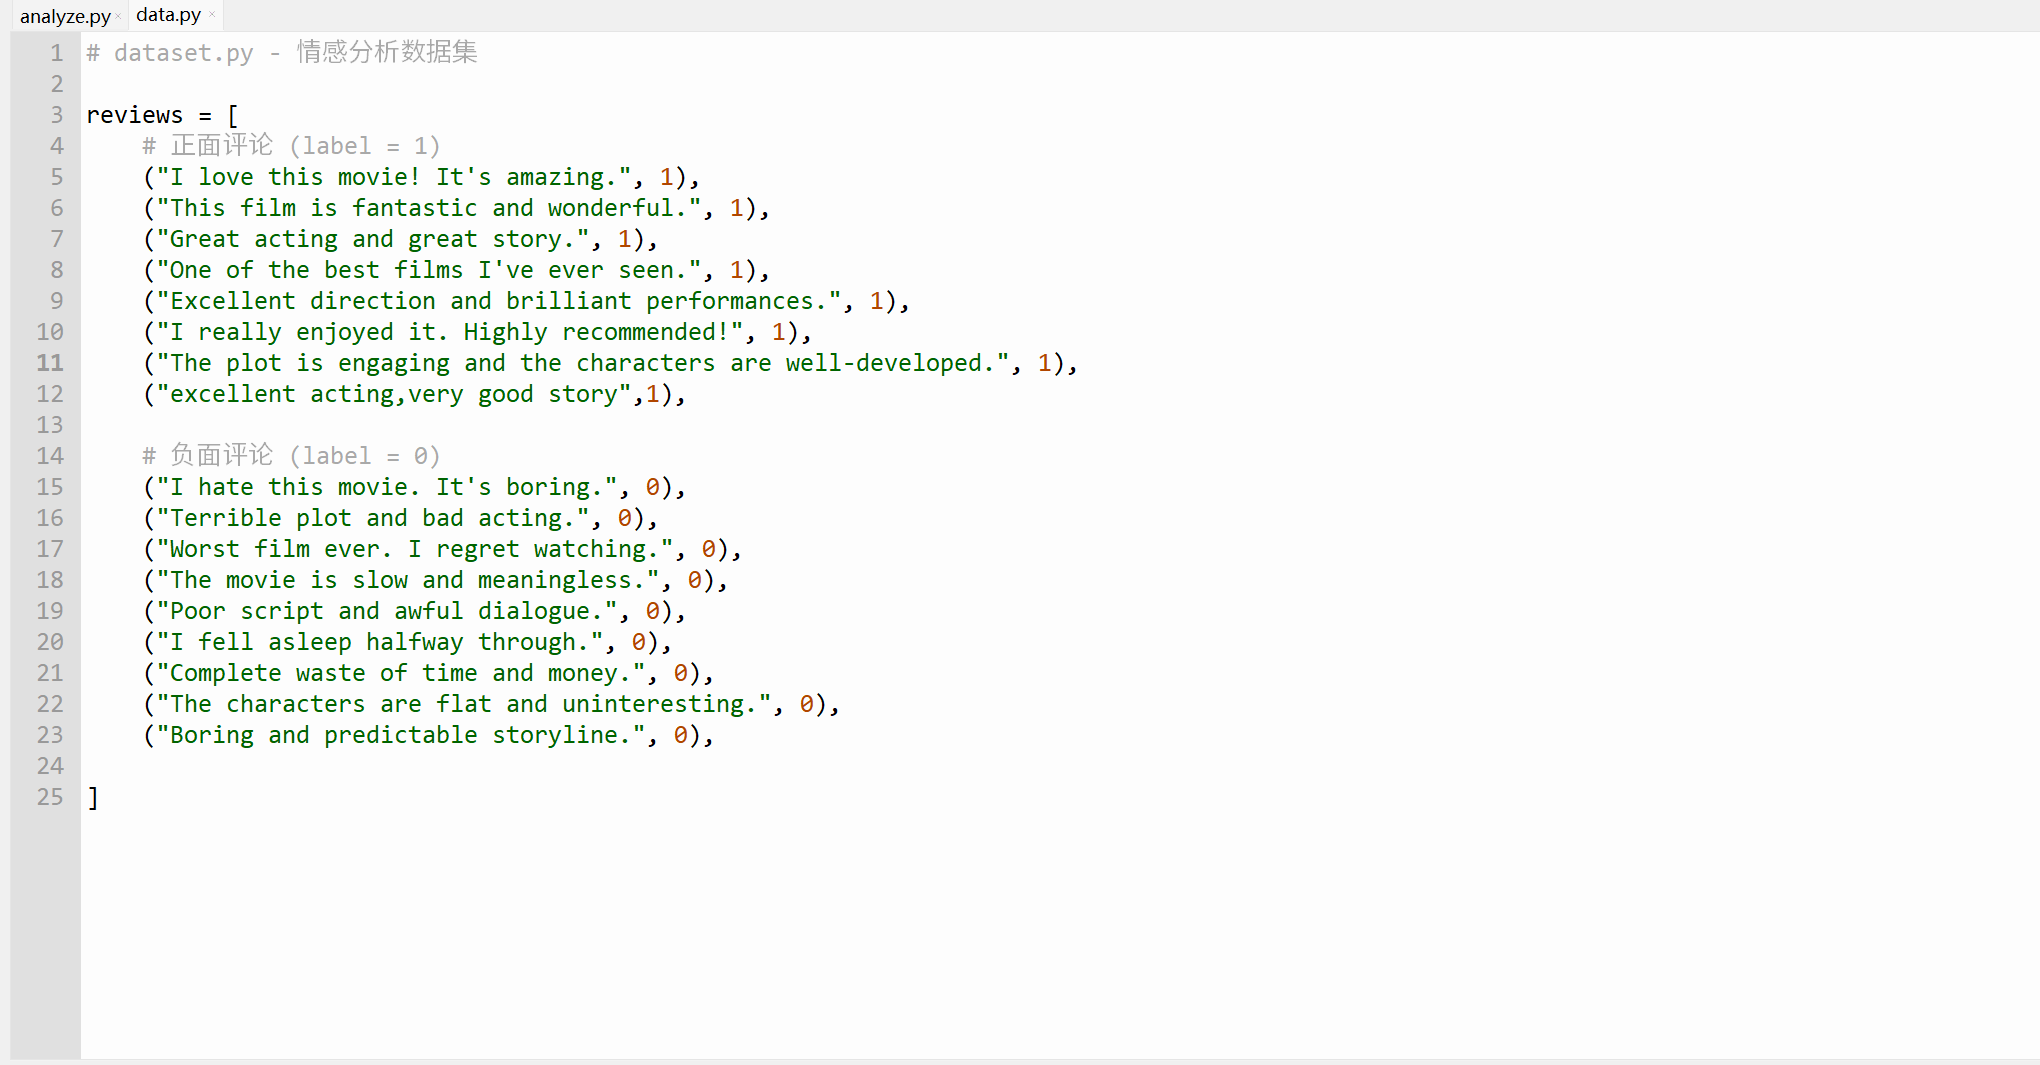
\includegraphics[width=0.8\textwidth]{lec4 (7).png}
    \caption{lec4-7}
\end{figure}

% 可选:如果你还有两张图需要展示(总共9张),可继续添加
\begin{figure}[htbp]
    \centering
    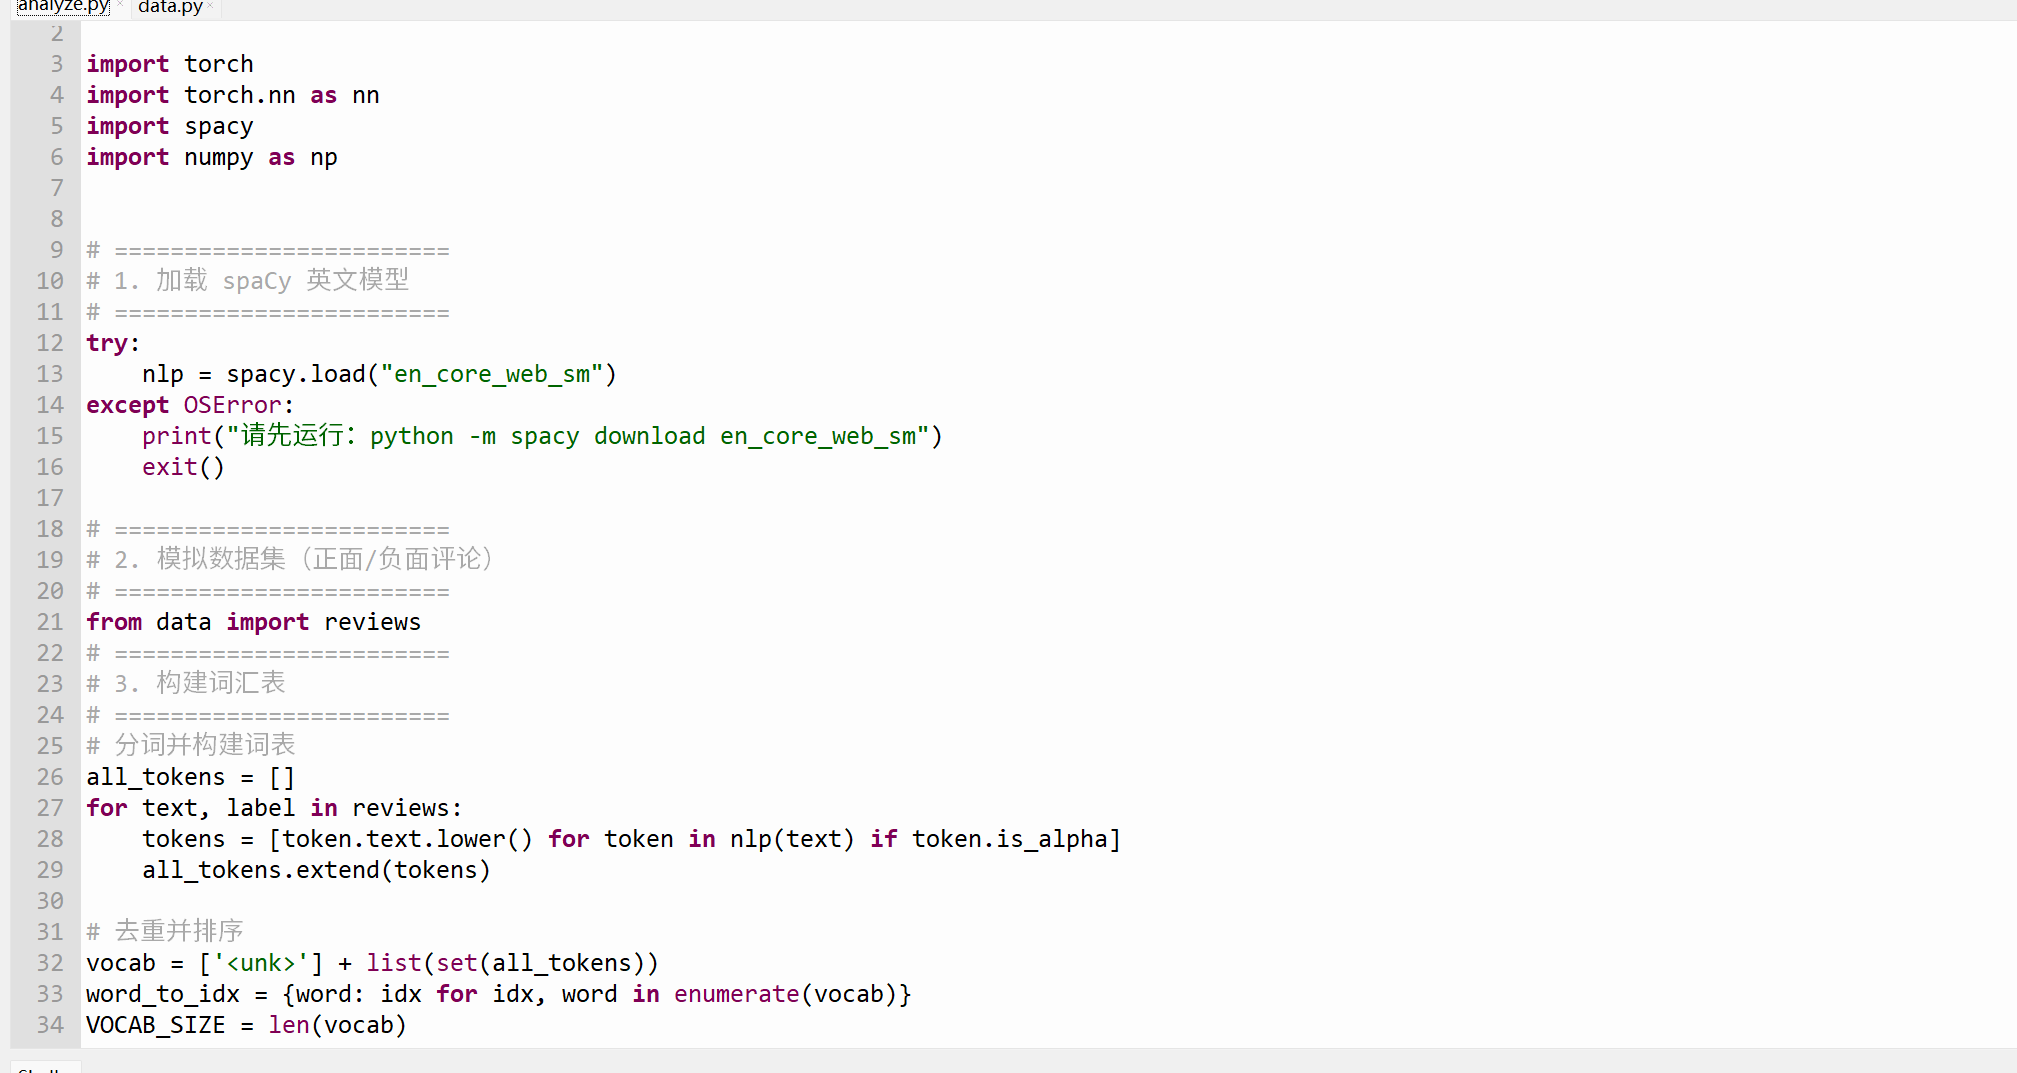
\includegraphics[width=0.8\textwidth]{lec4 (8).png}
    \caption{lec4-8}
\end{figure}

\begin{figure}[htbp]
    \centering
    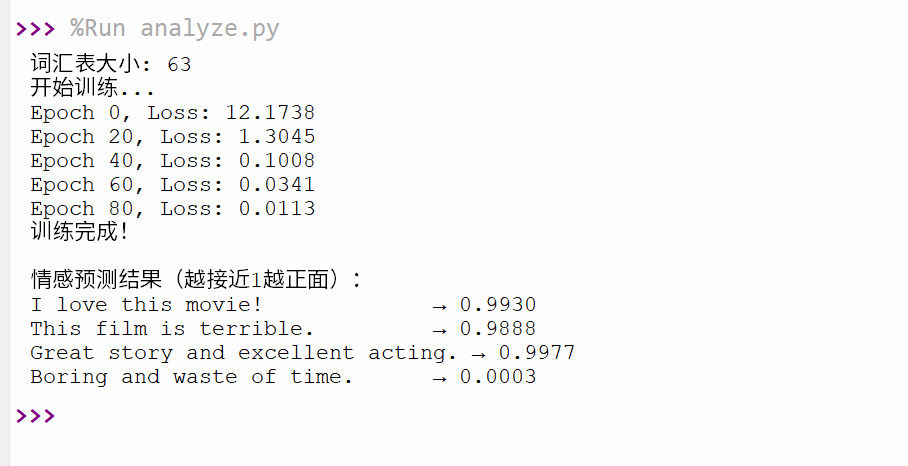
\includegraphics[width=0.8\textwidth]{lec4 (9).png}
    \caption{lec4-9}
\end{figure}

\newpage

\section*{五、实验结果}
\begin{itemize}
    \item 成功使用 \texttt{pdb} 对 Python 脚本进行断点调试,定位并修复了数据编码逻辑错误;
    \item 利用 \texttt{cProfile} 分析出模型训练中的性能瓶颈,优化了文本预处理流程;
    \item 编写 Makefile 实现了 LaTeX 文档的自动化编译,提升了文档构建效率;
    \item 构建了基于 PyTorch 的 LSTM 情感分析模型,训练后能对新句子进行合理的情感预测;
    \item 所有代码与文档已整理并提交至 GitHub 仓库https://github.com/ouc-lhy/for-lesson/tree/master/lesson4。
\end{itemize}

\section*{六、解题感悟}
本次实验深入掌握了软件开发中的关键技能:调试与性能分析。通过 \texttt{pdb},我学会了追踪程序执行流程,快速定位 bug。使用 \texttt{cProfile} 让我意识到性能优化的重要性。Makefile 与 LaTeX 的结合让我体会到"元编程"和自动化构建的强大。PyTorch 情感分析项目则让我初窥深度学习的魅力。这些技能不仅提升了我的编程能力,也培养了系统化思维,为后续课程和项目开发打下了坚实基础。

\section*{七、GitHub链接}
\url{https://github.com/ouc-lhy/for-lesson/tree/master/lesson4}

\end{document}